
\documentclass{beamer}

\mode<presentation> {
\usetheme{Madrid}
}
\usepackage{array}

\usepackage{graphicx}
\usepackage{subcaption}
\usepackage{booktabs}
\usepackage{url}
\usepackage{xcolor}
\usepackage{listings}
\usepackage{array}

\lstset{basicstyle=\ttfamily,
  showstringspaces=false,
  commentstyle=\color{red},
  keywordstyle=\color{blue},
}
%----------------------------------------------------------------------------------------
%	TITLE PAGE
%----------------------------------------------------------------------------------------

\title[InoXoft Bootcamp]{Go game winner prediction}
\author{Andrii Roiko} 
\institute[] 
{
\textit{Data-Focused Programming Bootcamp} \\\textit{InoXoft} \\ 
\medskip
\textit{roykoand@gmail.com}  
}

\AtBeginSection[]
{
  \begin{frame}<beamer>
    \frametitle{Content}
    \tableofcontents[currentsection]
  \end{frame}
}

\date{December 13, 2021} % Date, can be changed to a custom date

\begin{document}

\begin{frame}
\titlepage % Print the title page as the first slide
\end{frame}



%----------------------------------------------------------------------------------------
%	PRESENTATION SLIDES
%----------------------------------------------------------------------------------------


\section{Go game}
\begin{frame}
\frametitle{What is the Go/Weiqi/Baduk}


\begin{figure}
	\centering
	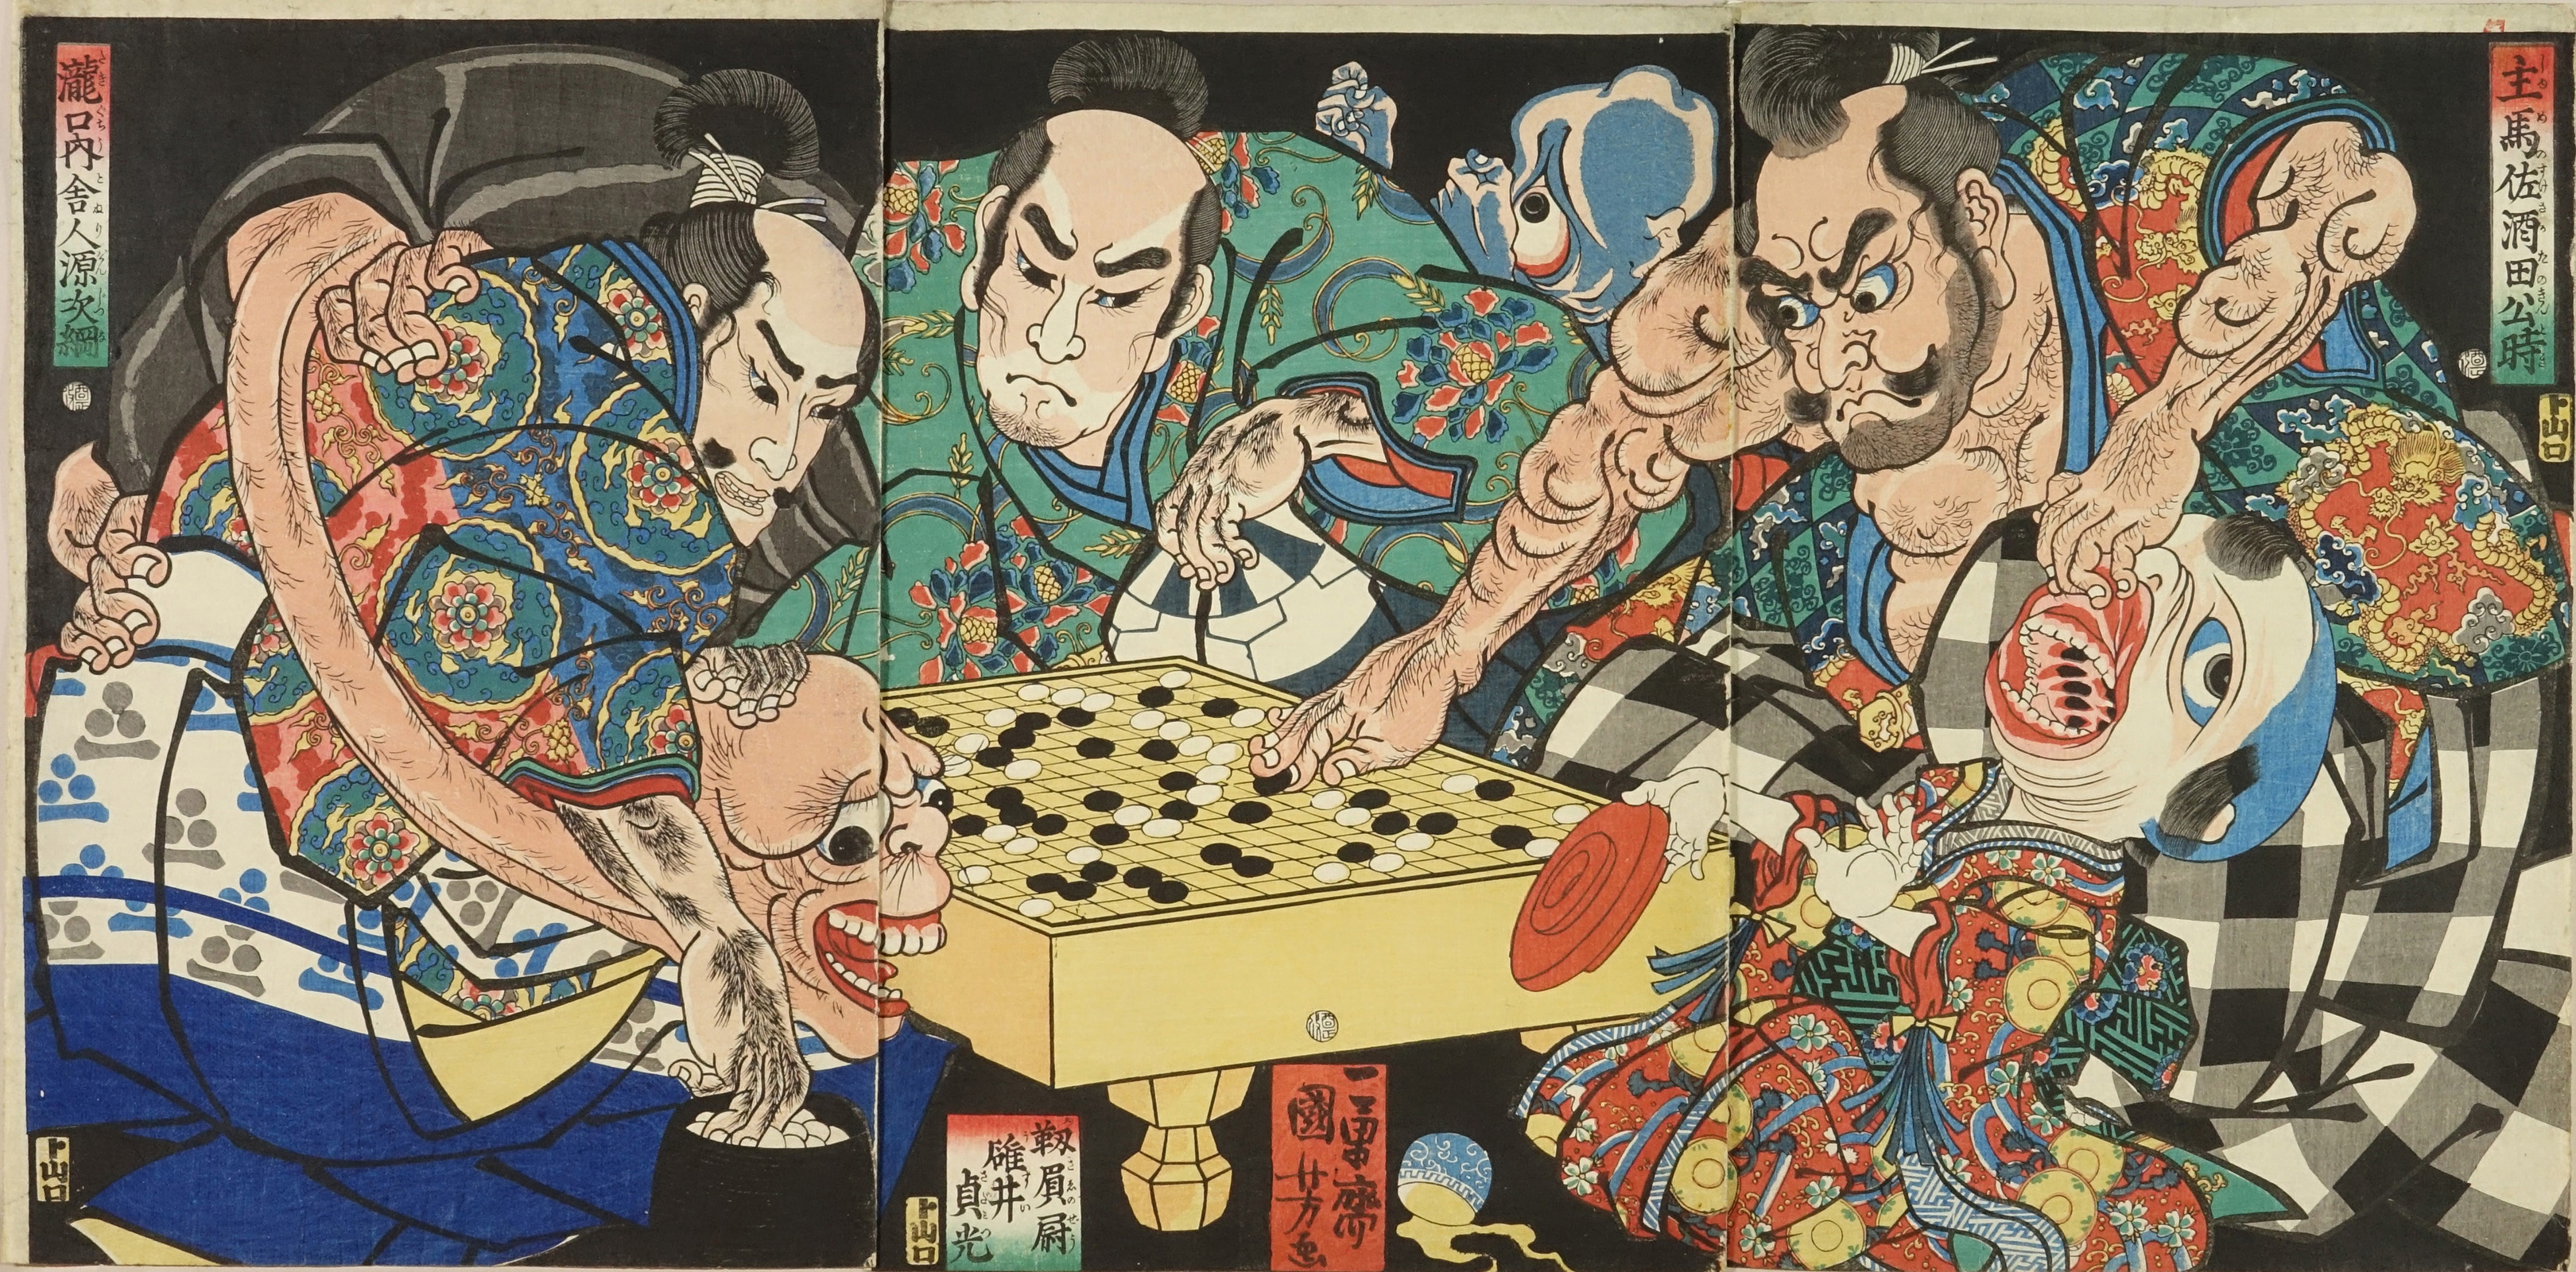
\includegraphics[scale=0.52]{images/gogame} 
	\caption*{Sakata Kintoki, Usui Sadamitsu, and Watanabe no Tsuna subdue monsters while playing go-game. Utagawa Kuniyoshi, 1861}
\end{figure}

\end{frame}

%------------------------------------------------
\begin{frame}
\frametitle{How to score a Game of Go}

Simplified formula of the total score (by Japanese rules):

\[Total\, score = \textbf{Prisoners} + ...\]

\end{frame}

%------------------------------------------------
\begin{frame}
\frametitle{Prisoners}

\begin{figure}
	\centering
	\includegraphics[scale=0.75]{images/prisoners}
	\caption*{Image was stolen from \url{https://www.kiseido.com/ff.html}}
\end{figure}


\end{frame}

%------------------------------------------------
\begin{frame}
\frametitle{How to score a Game of Go}

Simplified formula of the total score (by Japanese rules):

\[Total\, score = Prisoners + \textbf{Empty points} + ...\]

\end{frame}

%------------------------------------------------
\begin{frame}
\frametitle{Empty Points}

\begin{figure}
	\centering
	\includegraphics[scale=0.33]{images/scoring_territory}
	\caption*{Screenshot was made on \url{https://online-go.com}}
\end{figure}

\end{frame}

%------------------------------------------------
\begin{frame}
\frametitle{How to score a Game of Go}

Simplified formula of the total score (by Japanese rules):

\[Total\, score = Prisoners + Empty \, points + \textbf{Komi} \]

\end{frame}

%------------------------------------------------
\section{Problem definition}
\begin{frame}
\frametitle{Project goal}

\begin{figure}
	\centering
	\includegraphics[scale=0.28]{images/problem_def}
	\caption*{Screenshot was made on \url{https://online-go.com}}
\end{figure}

\end{frame}

%------------------------------------------------

\section{Dataset}
\begin{frame}[fragile]
\frametitle{Example of sgf file}

\begin{semiverbatim}
(;GM[1] FF[4] SZ[19] PW[vitality] WR[6d]
PB[Zeratul] BR[6d] DT[2008-12-05] 
PC[The KGS Go Server at http://www.gokgs.com/]
KM[6.50] RE[W+12.50] RU[Japanese] CA[UTF-8] ST[2] 
AP[CGoban:3] TM[60] OT[5x10 byo-yomi];
B[pd];W[dd];B[dp];W[pp];B[nq];W[qn];B[fc];W[hc];
B[cf];W[fd];B[cc];W[ec];B[cd];W[lq];B[fq];W[nc];
B[qf];W[pb];B[qc];W[ld];B[pq];W[qq];B[qr];W[oq];
B[pr];W[op];B[qp];W[rq];B[rp];W[rr];B[];W[])
\end{semiverbatim}

\end{frame}

%------------------------------------------------

\begin{frame}[fragile]
\frametitle{Example of sgf file}

\begin{semiverbatim}
(;GM[1] FF[4] SZ[19] PW[vitality] WR[6d]
PB[Zeratul] BR[6d] DT[2008-12-05] 
PC[The KGS Go Server at http://www.gokgs.com/]
KM[6.50] \textcolor{red}{RE[W+12.50]} RU[Japanese] CA[UTF-8] ST[2] 
AP[CGoban:3] TM[60] OT[5x10 byo-yomi];
\textcolor{red}{B[pd];W[dd];B[dp];W[pp];B[nq];W[qn];B[fc];W[hc];
B[cf];W[fd];B[cc];W[ec];B[cd];W[lq];B[fq];W[nc];
B[qf];W[pb];B[qc];W[ld];B[pq];W[qq];B[qr];W[oq];
B[pr];W[op];B[qp];W[rq];B[rp];W[rr];B[];W[])}
\end{semiverbatim}

\end{frame}

%------------------------------------------------

\begin{frame}[fragile]
\frametitle{SGF2PNG}

sgf2png utility: \url{https://github.com/julianandrews/sgf-render}

Dataset link: \url{https://bit.ly/31Urm46}

Total number of images: 30k [15k per class]

\begin{figure}
    \centering
     \caption*{Go board styles}
    \begin{subfigure}[b]{0.3\textwidth}
        \includegraphics[width=\textwidth]{images/style2.png}
        \caption*{Default board}
    \end{subfigure}
    \begin{subfigure}[b]{0.3\textwidth}
        \includegraphics[width=\textwidth]{images/style1.png}
        \caption*{Gradient stones}
    \end{subfigure}
    \begin{subfigure}[b]{0.3\textwidth}
        \includegraphics[width=\textwidth]{images/style3.png}
        \caption*{White-black board}
    \end{subfigure}
\end{figure}
	
\end{frame}

%------------------------------------------------

\section{Augmentation}
\begin{frame}
\frametitle{Types of input data}


\begin{figure}
    \centering
    \begin{subfigure}[b]{0.5\textwidth}
        \includegraphics[width=\textwidth]{images/input_type1.png}
        \caption*{Go board with background}
    \end{subfigure}
    \begin{subfigure}[b]{0.365\textwidth}
        \includegraphics[width=\textwidth]{images/input_type2.png}
        \caption*{Go board without background}
    \end{subfigure}
\end{figure}
	

\end{frame}

%------------------------------------------------

\begin{frame}
\frametitle{Augmentation}

\includegraphics[width=\textwidth]{images/background_example.png}


\end{frame}

%------------------------------------------------

\begin{frame}
\frametitle{Augmentation}
Backgrounds dataset: \url{https://www.kaggle.com/roykoandriy/go-apps-backgrounds}
\includegraphics[width=\textwidth]{images/background_example2.png}


\end{frame}

%------------------------------------------------

\begin{frame}
\frametitle{Augmentation}
Example of augmentation on different backgrounds:
\begin{center}
\includegraphics[scale=0.35]{images/augmentation.png}
\end{center}

\end{frame}

%------------------------------------------------

\begin{frame}
\frametitle{Augmentation}
Example of augmentation on different backgrounds:
\begin{center}
\includegraphics[scale=0.35]{images/augmentation_wb.png}
\end{center}

\end{frame}

%------------------------------------------------
\section{Model}
\begin{frame}
\frametitle{Optimization parameters and loss function}

\begin{center}
Loss function: Cross entropy

Optimizer: Adam (learning rate = $3 \cdot 10^{-4}$)

Learning rate scheduler: ReduceLROnPlateau
\end{center}

\end{frame}

%------------------------------------------------
\begin{frame}
\frametitle{DenseNet 121}

\begin{figure}
	\centering
	\includegraphics[scale=0.6]{images/model.png}
	\caption*{DenseNet models architecture} 
\end{figure}

\begin{center}
Densely Connected Convolutional Networks [\url{https://arxiv.org/abs/1608.06993}]
\end{center}

\end{frame}

%------------------------------------------------

\begin{frame}
\frametitle{Metrics on the test dataset}

\begin{center}
\begin{tabular}{ | c | c | } 
  \hline
Metric name & Score (percents) \\ 
  \hline
Accuracy & 73.9 \\ 
  \hline
Balanced accuracy & 73.9  \\ 
  \hline
F1 & 74.7  \\ 
  \hline
Precision & 75.3  \\ 
  \hline
Recall & 74.2 \\ 
  \hline
\end{tabular}
\\
*Test dataset metrics vary depending of the splitting
\end{center}

\end{frame}

%------------------------------------------------

\begin{frame}
\frametitle{Confusion matrix on the test dataset}

\begin{figure}
	\centering
	\includegraphics[scale=0.4]{images/confusion_matrix_td.png}
\end{figure}


\end{frame}

%------------------------------------------------

\begin{frame}
\frametitle{Predictions on the test dataset}

\begin{figure}
	\centering
	\includegraphics[scale=0.25]{images/predictions.png}
\end{figure}


\end{frame}

%------------------------------------------------

\section{Flask app}
\begin{frame}
\frametitle{Flask app}

\begin{center}
Path of the flask app in repository: 

\url{GoWinnerPrediction/app}
\end{center}

\end{frame}

%------------------------------------------------
\section{API}
\begin{frame}[fragile]
\frametitle{Go winner prediction API}
\begin{lstlisting}[basicstyle=\footnotesize, language=bash]
$ curl -X GET http://127.0.0.1:5000/?url=<URL_TO_THE_IMAGE>
{
    "prediction": "<COLOR_OF_THE_WINNER>",
    "url": "<URL_TO_THE_IMAGE>"
}
\end{lstlisting}

\end{frame}

%------------------------------------------------
\section{Links}
\begin{frame}
\frametitle{Links}

Github repo: \url{https://github.com/roykoand/GoWinnerPrediction}

This presentation in \url{GoWinnerPrediction/demo/presentation}

For inspiration (AlphaGo Documentary movie): \url{https://youtu.be/WXuK6gekU1Y}
\end{frame}

%------------------------------------------------

%------------------------------------------------

\begin{frame}
My contacts:
\begin{itemize}
\frametitle{The end :)}

\item Gmail: roykoand@gmail.com
\item Telegram: @roykoand
\item Github: \url{https://github.com/roykoand}
\item LinkedIn: \url{https://www.linkedin.com/in/roiko-andrii-3b330518a/}

\end{itemize}
\end{frame}

%----------------------------------------------------------------------------------------
\end{document} 